\section{Results}
\subsection{Gamma spectra (of four different sources)}
The MCA assigns all input signals to different channels based on their amplitudes, but no information is a priori known about which values of energy correspond to a certain channel.
Calibration is necessary to derive this relationship, which is linear
as the channels uniformly subdivide the total range of input values. \hl{Écrire mieux}

\hl{j'ai déplacé ce paragraphe dans la partie démarche exp, je pense qu'elle est mieux la bas}


This was accomplished using the known decay schemes\cite{notice_generale} of four radioactive sources: \cesium, \cobalt, \lead and \hafnium.
\footnote{Other sources were attempted (Sodium 22 and Cobalt 60), but their low count made for very long times to get reasonable spectrum.\hl{Enlever?}}

The $\gamma$ spectra of each of these sources were recorded and then gaussian fits were carried out on the the most recognisible peaks.
The bins corresponding to the averages of the obtained curves were associated with these known energies.

Figure \ref{fig:calibration_energy} shows the results of the calibration.
Linear as expected. Obtained factor of conversion.
\begin{figure}[htbp]
    \centering
    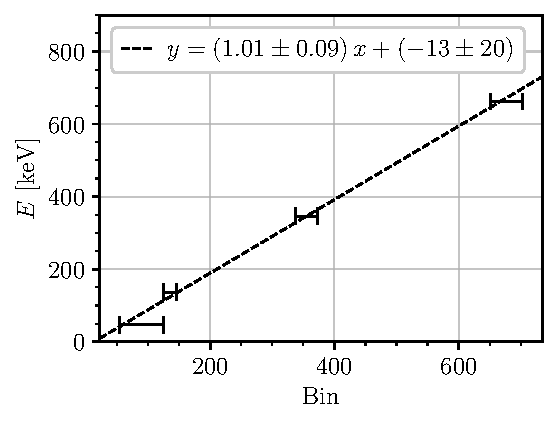
\includegraphics[scale=1]{figures/calibration_energy.pdf}
    \caption{Energy calibration of the spectrometer: known values of energies versus the channel in which they were registered by the MCA. \hl{Mieux écrire}}
    \label{fig:calibration_energy}
\end{figure}

Once the calibration was completed, it was possible to get gamma spectra of the four sources, with energies instead of bins.
See Figure \ref{fig:gamma_spectra}. Also other peaks were identified from decay schemes:
contribution from Compton is clearly visible here and there; collimation Lead.
\begin{figure}[htbp]
    \centering
    \begin{subfigure}{0.495\textwidth}
        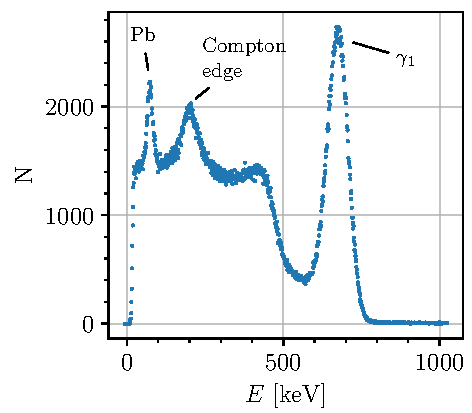
\includegraphics[scale=1]{figures/cs137_spectrum.pdf}
        \caption{}
    \end{subfigure}
    \hfill
    \begin{subfigure}{0.495\textwidth}
        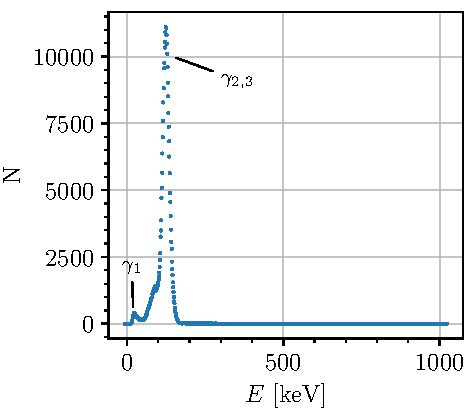
\includegraphics[scale=1]{figures/co57_spectrum.pdf}
        \caption{}
    \end{subfigure}
    \begin{subfigure}{0.495\textwidth}
        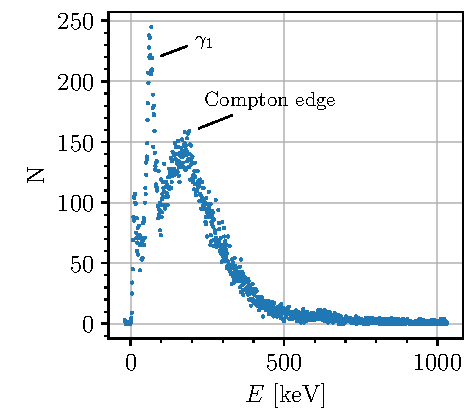
\includegraphics[scale=1]{figures/pb210_spectrum.pdf}
        \caption{}
    \end{subfigure}
    \hfill
    \begin{subfigure}{0.495\textwidth}
        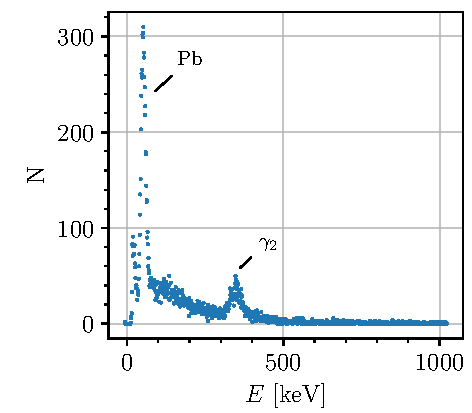
\includegraphics[scale=1]{figures/hf181_spectrum.pdf}
        \caption{}
    \end{subfigure}
    \caption{Gamma spectra of (a) $^{137}$Cs, (b) $^{57}$Co, (c) $^{210}$Pb, (d) $^{181}$Hf.}
    \label{fig:gamma_spectra}
\end{figure}


\subsection{Statistics}
It was discussed in Section ?? that decay follows a Poisson distribution, but as the mean gets higher the distribution tends to a gaussian one.
Two sets of measures were taken of the frequency of blabla.
\begin{figure}[htbp]
    \centering
    \begin{subfigure}{0.495\textwidth}
        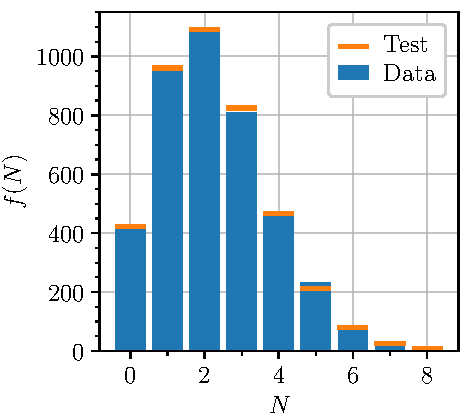
\includegraphics[scale=1]{figures/lowmean_poisson.pdf}
        \caption{}
    \end{subfigure}
    \hfill
    \begin{subfigure}{0.495\textwidth}
        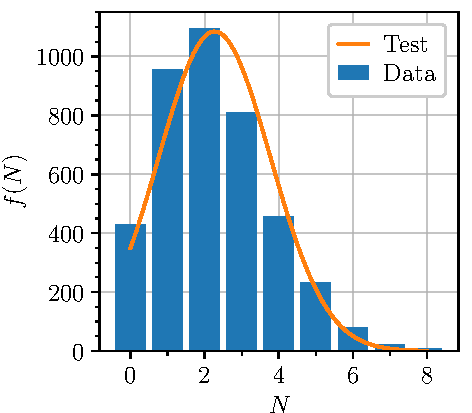
\includegraphics[scale=1]{figures/lowmean_gaussian.pdf}
        \caption{}
    \end{subfigure}
    \begin{subfigure}{0.495\textwidth}
        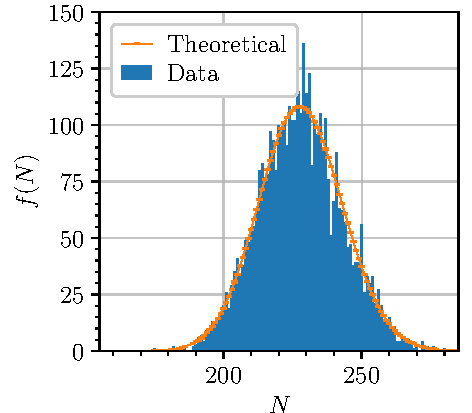
\includegraphics[scale=1]{figures/highmean_poisson.pdf}
        \caption{}
    \end{subfigure}
    \hfill
    \begin{subfigure}{0.495\textwidth}
        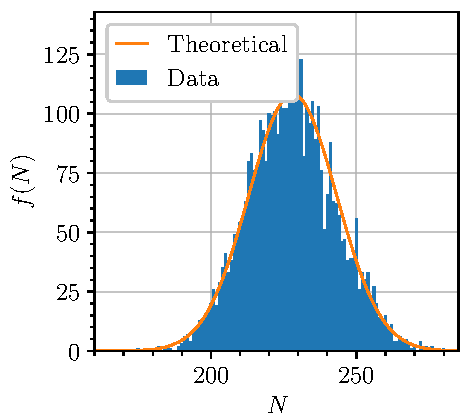
\includegraphics[scale=1]{figures/highmean_gaussian.pdf}
        \caption{}
    \end{subfigure}
    \caption{Results of the measurements of blabla and test distributions}
    \label{fig:statistical_tests}
\end{figure}

\begin{table}[htbp]
    \centering
    \begin{tabular}{lllllll}
        \hline
        Measure/dataset & Mean & Test distribution & $\nu$ & $p$-value & Result \\
        \hline
        \multirow{2}{*}{Low mean} & \multirow{2}{*}{2.27} & Poisson & 8 & 0.86 & Accepted\\
        & & Gaussian & 7 & $5.7 \times 10^{-117}$ & Rejected \\
        \multirow{2}{*}{High mean} & \multirow{2}{*}{228.10} & Poisson & 91 & 0.38 & Accepted\\
        & & Gaussian & 90 & 0.26 & Accepted\\
        \hline
    \end{tabular}
    \caption{[Characteristics] and results of the statistical tests carried out on two sets of datapoints? of different mean.}
    \label{tab:statistical_tests}
\end{table}

\paragraph{Attenuation in matter}
[We chose Cesium because of its high count rate].

Confirmed exponential nature of the attenuation.
The linear attenuation coefficient was found to be $\mu = (0.20 \pm 0.01)$ \unit{\per\cm} for Aluminium
and $\mu = (1.08 \pm 0.03)$ \unit{\per\cm} for Lead.
\begin{figure}[htbp]
    \centering
    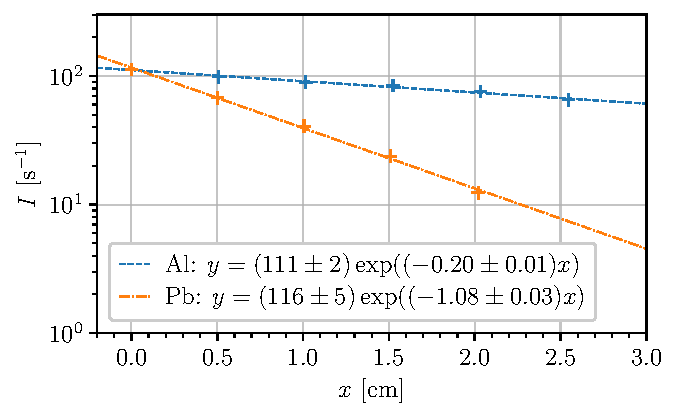
\includegraphics[scale=1]{figures/attenuation_coefficient.pdf}
    \caption{Radiation attenuation through Aluminum (Al) and Lead (Pb). 
             The error bars were omitted in reason of their small relative size 
             (1\% on the intensity and $1$ $\mu$m on the thickness of the material).}
    \label{fig:attenuation_coefficient}
\end{figure}


\paragraph{Resolution time of the coincidence selector}
\begin{figure}[htbp]
    \centering
    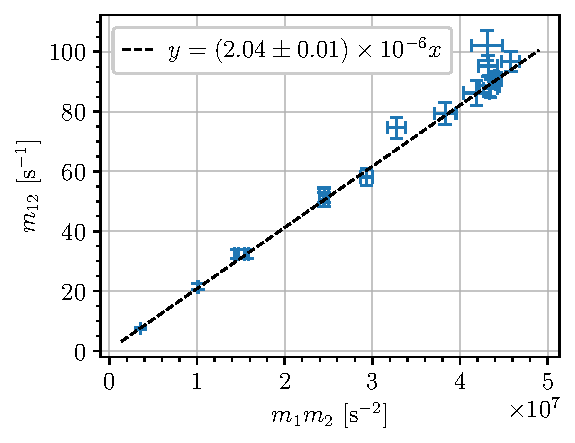
\includegraphics[scale=1]{figures/twotheta_cs137.pdf}
    \caption{\hl{Parler du cluster en haut à droite.}}
    \label{fig:twotheta_cs137}
\end{figure}

\paragraph{Co-57 activity}
Having determined the resolution time of the coincidence selector, an activity $A= (4127 \pm 53)$ Bq was obtained.